
In questa tesi, si andranno a studiare i funzionamenti delle reti private virtuali, delle necessità che portano alla loro installazione e si andrà a misurare le performance ottenute con diverse soluzioni software.
Prima di cominciare, è necessario fare un breve excursus definendo termini e concetti di base, fondamentali per comprendere i capitoli seguenti.

\section{Concetti di base}
\subsubsection{Server}
Un server è una macchina, un computer in grado di erogare servizi di ogni genere agli utenti (detti \emph{client}). Tendenzialmente, hanno potenze di calcolo superiori di vari ordini di grandezza rispetto ai dispositivi comunemente utilizzati, e fanno della ridondanza e dell'affidabilità pilastri fondamentali.

\subsubsection{Tipologie di reti}
Parlando di una rete di calcolatori, si intende una rete a cui sono connessi due o più computer tramite la quale è possibile condividere dati, dispositivi, connessione a internet, e via dicendo.

Esistono varie tipologie di reti di calcolatori, distinte in base al loro target, ossia all'estensione della rete.
Secondo questo parametro, è possibile distinguere le reti in Local Area Network (LAN), Metropolitan Area Network (MAN) e Wide Area Network (WAN). Tutte e tre le tipologie sono relative a una rete fisica.

Un altro tipo di reti è composto dalle reti private virtuali, o Virtual Private Networks (VPN), che consistono in reti di calcolatori le cui connessioni tra i nodi utilizzano reti pubbliche (WAN) come fondamenta su cui realizzare una rete virtuale.
Questo tipo di reti permette di realizzare collegamenti privati tra location geograficamente anche molto distanti senza la necessità di posare cavi fisici, ma avvalendosi dell'infrastruttura esistente, garantendo comunque integrità e cifratura dei dati, controllo degli accessi e confidenzialità.

\subsubsection{Il modello OSI}
\begin{figure}[ht]
    \centering
    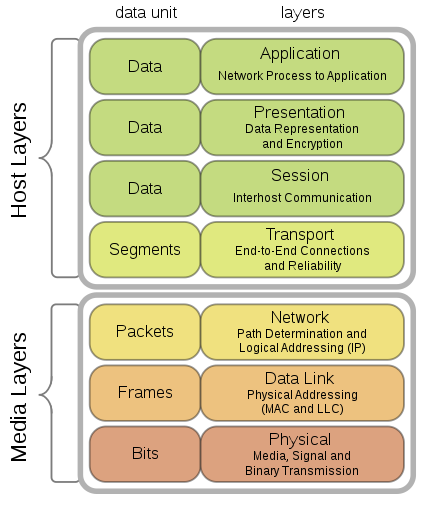
\includegraphics[width=10cm]{figure/osi.png}
    \caption{Modello OSI a strati}
\end{figure}

La pila ISO OSI è uno strumento estremamente efficace nel modellare il funzionamento di una rete di calcolatori.
Si basa su sette livelli, ognuno dei quali svolge il proprio lavoro utilizzando un'interfaccia standard offerta dal livello inferiore e offrendo a sua volta un'interfaccia al livello superiore.
Tutti e sette i livelli collaborano per rendere possibile il funzionamento della rete.

I compiti dei sette livelli sono, in breve, i seguenti:
\begin{enumerate}
    \item \textbf{Livello fisico}: è composto dall'infrastruttura fisica - cavi in rame, fibra ottica, ponti radio - e dai componenti hardware che codificano e decodificano i bit
    \item \textbf{Livello data-link}: si occupa di effettuare controlli sul livello fisico, specialmente sull'integrità dei dati
    \item \textbf{Livello di rete}: è il regno del protocollo IP, pilastro delle reti di calcolatori, che si occupa dello smistamento dei pacchetti e di portarli a destinazione; di particolare interesse sono gli indirizzi IP, che identificano in modo univoco un dispositivo collegato in rete
    \item \textbf{Livello di trasporto}: astrae il funzionamento del protocollo IP, offrendo alle applicazioni vari protocolli che si occupano della comunicazione tra due host, indipendentemente da come sono collegati o da quanto sono distanti; può garantire il recapito corretto delle informazioni
    \item \textbf{Livello di sessione, livello di presentazione, livello di applicazione}: sono gli strati più prossimi all'utente finale, e si occupano di gestire la comunicazione dei processi utilizzati dall'utente con il livello di trasporto
\end{enumerate}

% https://www.sciencedirect.com/topics/computer-science/security-architecture
\section{Pericoli di esporre un server su Internet}
Rendere accessibile un server dalla rete Internet, affinché sia possibile sfruttare i servizi che offre dovunque nel mondo ci si trovi, porta con sé una serie di rischi e problematiche concrete e decisamente rilevanti.
Infatti, i servizi pubblicati saranno esposti sia a utenti corretti che a malintenzionati, che potrebbero andare alla ricerca di vulnerabilità informatiche (ma non solo) col fine di ottenere accesso alle macchine e disporne a loro piacimento.


\section{Necessità di un'infrastruttura di rete sicura}
L'architettura di sicurezza del Modello OSI considera cinque classi principali di servizi di sicurezza. Tra queste si hanno: autenticazione, controllo degli accessi, confidenzialità, integrità e non ripudio.
In particolare, questi servizi sono definiti come segue:
\begin{itemize}
    \item \textbf{autenticazione} - il servizio di autenticazione verifica l'identità di un utente o di un sistema
    \item \textbf{controllo degli accessi} - il servizio protegge le risorse di sistema da utenti non autorizzati
    \item \textbf{confidenzialità} - il servizio protegge i dati da rivelazioni non autorizzate
    \item \textbf{integrità} - il servizio protegge i dati da modifiche, aggiunte o rimozioni non autorizzate
    \item \textbf{non ripudio} \emph{a.k.a non-repudiation} - il servizio assicura che il mittente dell'informazione abbia una notifica di consegna e il destinatario riceva una prova di identità del mittente, in modo tale che nessuno dei due possa successivamente negare di aver processato tali dati
\end{itemize}
Un'architettura sicura deve garantire tutti e cinque i servizi.

\section{Organizzazione dei capitoli}
I capitoli che seguono sono sviluppati come segue.

Nel capitolo $1$, vengono discussi i requisiti del sistema che andranno rispettati nello svolgimento della tesi.

Nel capitolo $2$, si discute lo stato dell'arte, illustrando dal punto di vista teorico i protocolli e i software che si andranno a utilizzare.

Nel capitolo $3$, viene illustrata la realizzazione dell'ambiente di test, compresa l'installazione e la configurazione dei servizi scelti.

Nel capitolo $4$, si analizzano le misure ottenute durante i test.

Nel capitolo $5$, si presentano i principali problemi di sicurezza a cui si potrebbe andare incontro.

